\documentclass{standalone}
\usepackage{tikz}
\usetikzlibrary{patterns, positioning}


\begin{document}
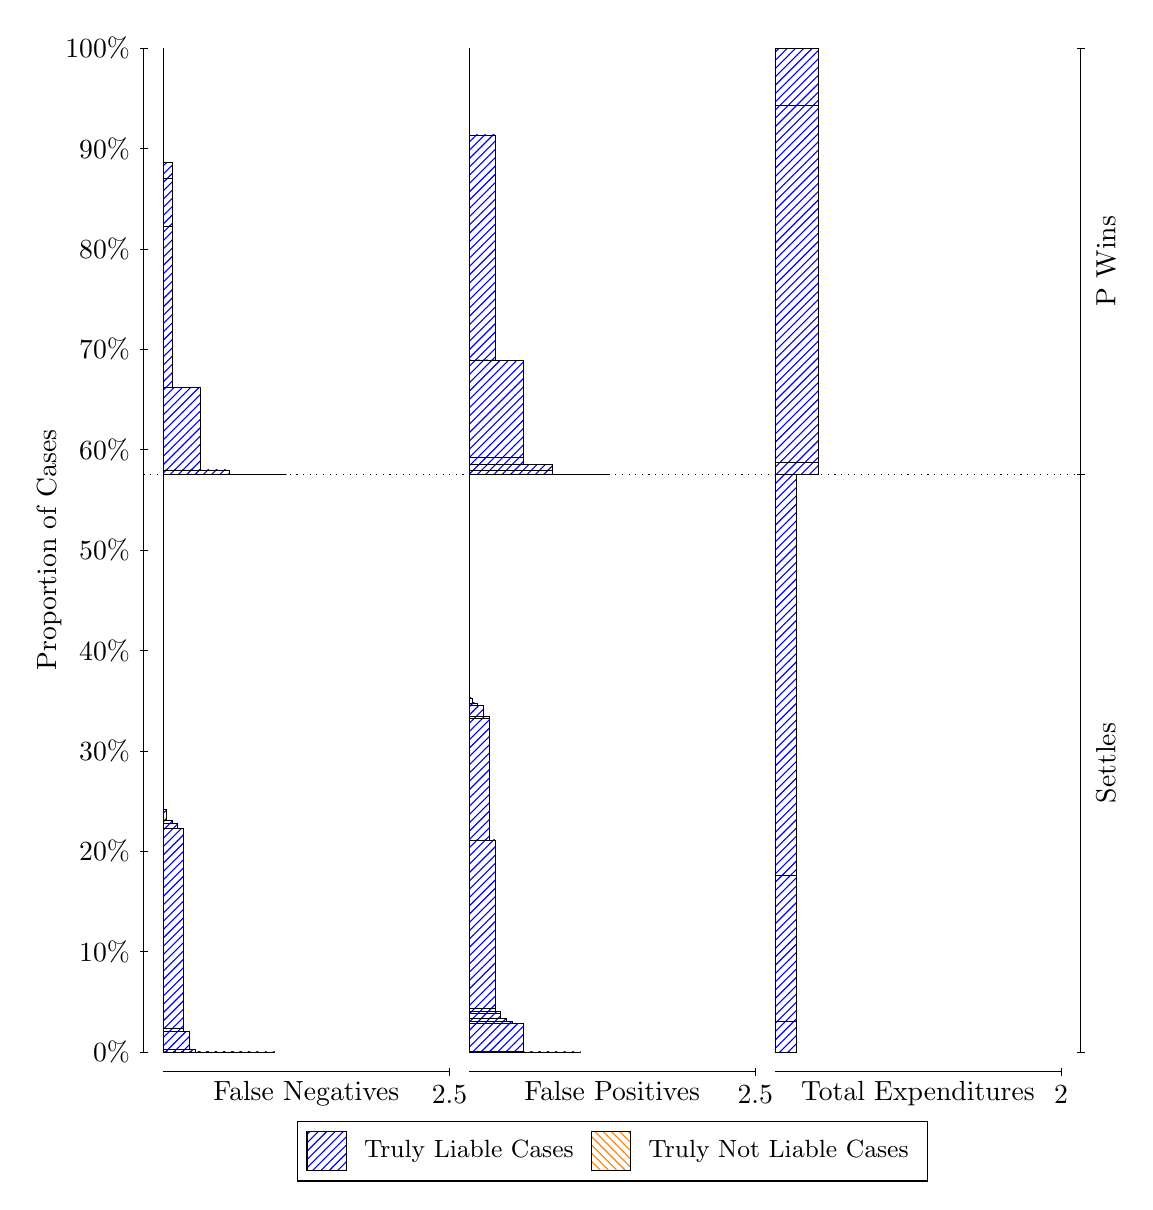
\begin{tikzpicture}
\draw[black, very thin] (1.5,1.75) -- (1.5,14.5);
\node[rotate=90, text=black, anchor=center] at (0.3, 8.125) {Proportion of Cases};
\draw[black, very thin] (1.45,1.75) -- (1.55,1.75);
\node[text=black, anchor=east] at (1.45, 1.75) {0\%};
\draw[black, very thin] (1.45,3.025) -- (1.55,3.025);
\node[text=black, anchor=east] at (1.45, 3.025) {10\%};
\draw[black, very thin] (1.45,4.3) -- (1.55,4.3);
\node[text=black, anchor=east] at (1.45, 4.3) {20\%};
\draw[black, very thin] (1.45,5.575) -- (1.55,5.575);
\node[text=black, anchor=east] at (1.45, 5.575) {30\%};
\draw[black, very thin] (1.45,6.85) -- (1.55,6.85);
\node[text=black, anchor=east] at (1.45, 6.85) {40\%};
\draw[black, very thin] (1.45,8.125) -- (1.55,8.125);
\node[text=black, anchor=east] at (1.45, 8.125) {50\%};
\draw[black, very thin] (1.45,9.4) -- (1.55,9.4);
\node[text=black, anchor=east] at (1.45, 9.4) {60\%};
\draw[black, very thin] (1.45,10.675) -- (1.55,10.675);
\node[text=black, anchor=east] at (1.45, 10.675) {70\%};
\draw[black, very thin] (1.45,11.95) -- (1.55,11.95);
\node[text=black, anchor=east] at (1.45, 11.95) {80\%};
\draw[black, very thin] (1.45,13.225) -- (1.55,13.225);
\node[text=black, anchor=east] at (1.45, 13.225) {90\%};
\draw[black, very thin] (1.45,14.5) -- (1.55,14.5);
\node[text=black, anchor=east] at (1.45, 14.5) {100\%};

\draw[black, very thin] (13.4,1.75) -- (13.4,14.5);
\draw[black, very thin] (13.35,1.75) -- (13.45,1.75);
\node[anchor=west] at (13.35, 1.75) {};
\draw[black, very thin] (13.35,9.0884) -- (13.45,9.0884);
\node[anchor=west] at (13.35, 9.0884) {};
\draw[black, very thin] (13.35,14.5) -- (13.45,14.5);
\node[anchor=west] at (13.35, 14.5) {};

\draw[black, very thin, pattern color=blue, pattern=north east lines] (1.75,1.75) rectangle (3.167,1.75);
\draw[black, very thin, pattern color=blue, pattern=north east lines] (1.75,1.75) rectangle (3.0217,1.75);
\draw[black, very thin, pattern color=blue, pattern=north east lines] (1.75,1.75) rectangle (2.8763,1.75);
\draw[black, very thin, pattern color=blue, pattern=north east lines] (1.75,1.75) rectangle (2.8037,1.75);
\draw[black, very thin, pattern color=blue, pattern=north east lines] (1.75,1.75) rectangle (2.731,1.75);
\draw[black, very thin, pattern color=blue, pattern=north east lines] (1.75,1.75) rectangle (2.6583,1.75);
\draw[black, very thin, pattern color=blue, pattern=north east lines] (1.75,1.75) rectangle (2.5857,1.75);
\draw[black, very thin, pattern color=blue, pattern=north east lines] (1.75,1.75) rectangle (2.513,1.75);
\draw[black, very thin, pattern color=blue, pattern=north east lines] (1.75,1.75) rectangle (2.4403,1.7511);
\draw[black, very thin, pattern color=blue, pattern=north east lines] (1.75,1.7511) rectangle (2.3677,1.7511);
\draw[black, very thin, pattern color=blue, pattern=north east lines] (1.75,1.7511) rectangle (2.295,1.7517);
\draw[black, very thin, pattern color=blue, pattern=north east lines] (1.75,1.7517) rectangle (2.2223,1.7518);
\draw[black, very thin, pattern color=blue, pattern=north east lines] (1.75,1.7518) rectangle (2.1497,1.781);
\draw[black, very thin, pattern color=blue, pattern=north east lines] (1.75,1.781) rectangle (2.077,2.0161);
\draw[black, very thin, pattern color=blue, pattern=north east lines] (1.75,2.0161) rectangle (2.0043,2.0458);
\draw[black, very thin, pattern color=blue, pattern=north east lines] (1.75,2.0458) rectangle (2.0043,4.5917);
\draw[black, very thin, pattern color=blue, pattern=north east lines] (1.75,4.5917) rectangle (1.9317,4.6539);
\draw[black, very thin, pattern color=blue, pattern=north east lines] (1.75,4.6539) rectangle (1.859,4.6898);
\draw[black, very thin, pattern color=blue, pattern=north east lines] (1.75,4.6898) rectangle (1.7863,4.8306);
\draw[black, very thin, pattern color=orange, pattern=north west lines] (1.75,4.8306) rectangle (1.75,4.8306);
\draw[black, very thin, pattern color=blue, pattern=north east lines] (1.75,4.8306) rectangle (1.75,9.0884);
\draw[black, very thin, pattern color=blue, pattern=north east lines] (1.75,9.0884) rectangle (3.3123,9.0884);
\draw[black, very thin, pattern color=blue, pattern=north east lines] (1.75,9.0884) rectangle (2.949,9.0885);
\draw[black, very thin, pattern color=blue, pattern=north east lines] (1.75,9.0885) rectangle (2.5857,9.1437);
\draw[black, very thin, pattern color=blue, pattern=north east lines] (1.75,9.1437) rectangle (2.2223,10.19);
\draw[black, very thin, pattern color=blue, pattern=north east lines] (1.75,10.19) rectangle (2.2223,10.191);
\draw[black, very thin, pattern color=blue, pattern=north east lines] (1.75,10.191) rectangle (1.859,12.24);
\draw[black, very thin, pattern color=blue, pattern=north east lines] (1.75,12.24) rectangle (1.859,12.844);
\draw[black, very thin, pattern color=blue, pattern=north east lines] (1.75,12.844) rectangle (1.859,13.052);
\draw[black, very thin, pattern color=orange, pattern=north west lines] (1.75,13.052) rectangle (1.75,13.052);
\draw[black, very thin, pattern color=blue, pattern=north east lines] (1.75,13.052) rectangle (1.75,14.5);
\draw[black, very thin, pattern color=orange, pattern=north west lines] (5.6333,1.75) rectangle (7.0503,1.75);
\draw[black, very thin, pattern color=blue, pattern=north east lines] (5.6333,1.75) rectangle (7.0503,1.75);
\draw[black, very thin, pattern color=orange, pattern=north west lines] (5.6333,1.75) rectangle (6.7597,1.75);
\draw[black, very thin, pattern color=blue, pattern=north east lines] (5.6333,1.75) rectangle (6.7597,1.75);
\draw[black, very thin, pattern color=blue, pattern=north east lines] (5.6333,1.75) rectangle (6.687,1.7513);
\draw[black, very thin, pattern color=orange, pattern=north west lines] (5.6333,1.7513) rectangle (6.6143,1.7513);
\draw[black, very thin, pattern color=blue, pattern=north east lines] (5.6333,1.7513) rectangle (6.6143,1.7513);
\draw[black, very thin, pattern color=orange, pattern=north west lines] (5.6333,1.7513) rectangle (6.469,1.7513);
\draw[black, very thin, pattern color=blue, pattern=north east lines] (5.6333,1.7513) rectangle (6.469,1.7514);
\draw[black, very thin, pattern color=blue, pattern=north east lines] (5.6333,1.7514) rectangle (6.3963,1.7523);
\draw[black, very thin, pattern color=orange, pattern=north west lines] (5.6333,1.7523) rectangle (6.3237,1.7523);
\draw[black, very thin, pattern color=blue, pattern=north east lines] (5.6333,1.7523) rectangle (6.3237,1.7526);
\draw[black, very thin, pattern color=blue, pattern=north east lines] (5.6333,1.7526) rectangle (6.3237,2.1129);
\draw[black, very thin, pattern color=blue, pattern=north east lines] (5.6333,2.1129) rectangle (6.251,2.1137);
\draw[black, very thin, pattern color=orange, pattern=north west lines] (5.6333,2.1137) rectangle (6.1783,2.1137);
\draw[black, very thin, pattern color=blue, pattern=north east lines] (5.6333,2.1137) rectangle (6.1783,2.14);
\draw[black, very thin, pattern color=blue, pattern=north east lines] (5.6333,2.14) rectangle (6.1057,2.176);
\draw[black, very thin, pattern color=orange, pattern=north west lines] (5.6333,2.176) rectangle (6.033,2.176);
\draw[black, very thin, pattern color=blue, pattern=north east lines] (5.6333,2.176) rectangle (6.033,2.2434);
\draw[black, very thin, pattern color=blue, pattern=north east lines] (5.6333,2.2434) rectangle (6.033,2.2672);
\draw[black, very thin, pattern color=blue, pattern=north east lines] (5.6333,2.2672) rectangle (5.9603,2.3017);
\draw[black, very thin, pattern color=blue, pattern=north east lines] (5.6333,2.3017) rectangle (5.9603,4.4446);
\draw[black, very thin, pattern color=orange, pattern=north west lines] (5.6333,4.4446) rectangle (5.8877,4.4446);
\draw[black, very thin, pattern color=blue, pattern=north east lines] (5.6333,4.4446) rectangle (5.8877,5.9877);
\draw[black, very thin, pattern color=blue, pattern=north east lines] (5.6333,5.9877) rectangle (5.8877,6.0077);
\draw[black, very thin, pattern color=blue, pattern=north east lines] (5.6333,6.0077) rectangle (5.815,6.1486);
\draw[black, very thin, pattern color=blue, pattern=north east lines] (5.6333,6.1486) rectangle (5.7423,6.1845);
\draw[black, very thin, pattern color=blue, pattern=north east lines] (5.6333,6.1845) rectangle (5.6697,6.2456);
\draw[black, very thin, pattern color=blue, pattern=north east lines] (5.6333,6.2456) rectangle (5.6697,6.2467);
\draw[black, very thin, pattern color=blue, pattern=north east lines] (5.6333,6.2467) rectangle (5.6333,9.0884);
\draw[black, very thin, pattern color=orange, pattern=north west lines] (5.6333,9.0884) rectangle (7.4137,9.0884);
\draw[black, very thin, pattern color=blue, pattern=north east lines] (5.6333,9.0884) rectangle (7.4137,9.0884);
\draw[black, very thin, pattern color=blue, pattern=north east lines] (5.6333,9.0884) rectangle (7.0503,9.0893);
\draw[black, very thin, pattern color=orange, pattern=north west lines] (5.6333,9.0893) rectangle (7.0503,9.0893);
\draw[black, very thin, pattern color=blue, pattern=north east lines] (5.6333,9.0893) rectangle (7.0503,9.0898);
\draw[black, very thin, pattern color=blue, pattern=north east lines] (5.6333,9.0898) rectangle (6.687,9.1356);
\draw[black, very thin, pattern color=orange, pattern=north west lines] (5.6333,9.1356) rectangle (6.687,9.1356);
\draw[black, very thin, pattern color=blue, pattern=north east lines] (5.6333,9.1356) rectangle (6.687,9.2094);
\draw[black, very thin, pattern color=blue, pattern=north east lines] (5.6333,9.2094) rectangle (6.3237,9.3046);
\draw[black, very thin, pattern color=orange, pattern=north west lines] (5.6333,9.3046) rectangle (6.3237,9.3046);
\draw[black, very thin, pattern color=blue, pattern=north east lines] (5.6333,9.3046) rectangle (6.3237,10.536);
\draw[black, very thin, pattern color=blue, pattern=north east lines] (5.6333,10.536) rectangle (5.9603,10.539);
\draw[black, very thin, pattern color=orange, pattern=north west lines] (5.6333,10.539) rectangle (5.9603,10.539);
\draw[black, very thin, pattern color=blue, pattern=north east lines] (5.6333,10.539) rectangle (5.9603,13.397);
\draw[black, very thin, pattern color=blue, pattern=north east lines] (5.6333,13.397) rectangle (5.6333,14.5);
\draw[black, very thin, pattern color=orange, pattern=north west lines] (9.5167,1.75) rectangle (9.7892,1.75);
\draw[black, very thin, pattern color=blue, pattern=north east lines] (9.5167,1.75) rectangle (9.7892,2.14);
\draw[black, very thin, pattern color=orange, pattern=north west lines] (9.5167,2.14) rectangle (9.7892,2.14);
\draw[black, very thin, pattern color=blue, pattern=north east lines] (9.5167,2.14) rectangle (9.7892,3.9904);
\draw[black, very thin, pattern color=orange, pattern=north west lines] (9.5167,3.9904) rectangle (9.7892,3.9904);
\draw[black, very thin, pattern color=blue, pattern=north east lines] (9.5167,3.9904) rectangle (9.7892,9.0884);
\draw[black, very thin, pattern color=orange, pattern=north west lines] (9.5167,9.0884) rectangle (10.062,9.0884);
\draw[black, very thin, pattern color=blue, pattern=north east lines] (9.5167,9.0884) rectangle (10.062,9.2329);
\draw[black, very thin, pattern color=orange, pattern=north west lines] (9.5167,9.2329) rectangle (10.062,9.2329);
\draw[black, very thin, pattern color=blue, pattern=north east lines] (9.5167,9.2329) rectangle (10.062,13.775);
\draw[black, very thin, pattern color=orange, pattern=north west lines] (9.5167,13.775) rectangle (10.062,13.775);
\draw[black, very thin, pattern color=blue, pattern=north east lines] (9.5167,13.775) rectangle (10.062,14.5);
\draw[black, dotted] (1.5,9.0884) -- (13.4,9.0884);
\draw[black, very thin] (1.75,1.5) -- (5.3833,1.5);
\node[text=black, anchor=north] at (3.5667, 1.5) {False Negatives};
\draw[black, very thin] (5.3833,1.45) -- (5.3833,1.55);
\node[text=black, anchor=north] at (5.3833, 1.45) {2.5};

\draw[black, very thin] (5.6333,1.5) -- (9.2667,1.5);
\node[text=black, anchor=north] at (7.45, 1.5) {False Positives};
\draw[black, very thin] (9.2667,1.45) -- (9.2667,1.55);
\node[text=black, anchor=north] at (9.2667, 1.45) {2.5};

\draw[black, very thin] (9.5167,1.5) -- (13.15,1.5);
\node[text=black, anchor=north] at (11.333, 1.5) {Total Expenditures};
\draw[black, very thin] (13.15,1.45) -- (13.15,1.55);
\node[text=black, anchor=north] at (13.15, 1.45) {2};

\node[text=black, centered, rotate=90] at (13.72, 5.4192) {Settles};
\node[text=black, centered, rotate=90] at (13.72, 11.794) {P Wins};

\draw (7.449999999999999,1.5) node[draw=none] (baseCoordinate) {};
\begin{scope}[align=center]
        \matrix[scale=0.5, draw=black, below=0.5cm of baseCoordinate, nodes={draw}, column sep=0.1cm]{
            \node[rectangle, draw, minimum width=0.5cm, minimum height=0.5cm, pattern color=blue, pattern=north east lines] {}; &
            \node[draw=none, font=\small, text=black] (B) {Truly Liable Cases}; &
            \node[rectangle, draw, minimum width=0.5cm, minimum height=0.5cm, pattern color=orange, pattern=north west lines] {}; &
            \node[draw=none, font=\small, text=black] (B) {Truly Not Liable Cases}; \\
            };
\end{scope}

\end{tikzpicture}
\end{document}